\documentclass[11pt]{article}

\usepackage[a4paper, margin=2.5cm]{geometry}
\usepackage{amsmath, amssymb}
\usepackage{graphicx}
\usepackage{hyperref}
\usepackage{natbib}
\usepackage{caption}
\usepackage{subcaption}

\title{
Absence of Structural Phase Transition but Emergence of Heavy-Tailed Statistics \\
in Spin Glass Landscapes Controlled by Kurtosis
}

\author{Eduardo Gonzalez-Granda Fernandez\\
\textit{Independent Researcher, Salamanca, Spain}\\
\href{mailto:eggranda@usal.es}{eggranda@usal.es}\\
\href{https://orcid.org/0000-0002-6771-5145}{ORCID: 0000-0002-6771-5145}
}
\date{\today \\ \vspace{0.4cm} 
\textbf{DOI:} \href{https://doi.org/10.5281/10.5281/zenodo.19593591}{10.5281/zenodo.19593591}}
\begin{document}

\maketitle

\begin{abstract}

Recent work on latent generative models (GLG) has revealed a sharp phase transition in structural complexity as a function of kurtosis, suggesting a form of universality \citep{gonzalez2023m18}. In this work, we test this hypothesis in a fundamentally different class of systems: spin glass energy landscapes \citep{mezard1987spin, binder1986spin}.

We show that, unlike GLG, spin glass systems do not exhibit any structural phase transition when varying the kurtosis of coupling distributions. Global observables such as the number of local minima, effective dimensionality, and energy landscape roughness remain invariant across a wide range of kurtosis values.

However, we uncover a distinct statistical transition: the distribution of energy gaps develops heavy tails, transitioning from approximately log-normal behavior at low kurtosis to power-law behavior at high kurtosis. The global tail is well described by a power law with exponent $\alpha \approx 2.5$.

These results demonstrate that kurtosis does not universally induce structural reorganization, but instead controls the statistics of rare events in disordered systems. This establishes a clear boundary for the domain of validity of kurtosis-driven universality.

\end{abstract}

\section{Introduction}

The emergence of macroscopic structure from microscopic randomness is a central theme in statistical physics and complex systems. Recent results in latent generative graph models (GLG) have shown that increasing kurtosis in latent distributions induces a sharp transition in structural complexity, characterized by a sigmoid collapse in effective dimensionality \citep{gonzalez2023m18}.

This has been interpreted as evidence of a universal phase transition controlled by kurtosis.

The goal of this work is to test this hypothesis in a different class of systems: spin glass energy landscapes \citep{young1998spin, talagrand2003spin}. Unlike generative models, spin glasses are defined by quenched disorder and frustrated interactions, leading to highly rugged energy landscapes \citep{derrida1980random, derrida1981random}.

The central question is:

\begin{quote}
Does kurtosis induce a structural phase transition in spin glass systems?
\end{quote}

\section{Methods}

We generate ensembles of spin glass instances with coupling distributions of varying kurtosis $\kappa$, including Gaussian, Laplace, and heavy-tailed distributions.

For each instance, we compute:

\begin{itemize}
\item Number of local minima $n_{\min}$
\item Energy gap $\Delta E = E_2 - E_1$
\item Energy landscape roughness (standard deviation of energies)
\item Effective dimensionality $d_G$ via PCA
\end{itemize}

A total of 617 instances are analyzed, covering a kurtosis range:

\[
\kappa \in [0.005, 83.567]
\]

Energy gaps include a significant fraction of exact degeneracies:

\[
\text{fraction of } \Delta E = 0 \approx 0.436
\]

Heavy-tail analysis is performed using maximum likelihood estimation \citep{clauset2009power, newman2005power}, comparing:

\begin{itemize}
\item Power law: $p(x) \sim x^{-\alpha}$
\item Log-normal: $p(x) \sim \exp(-(\log x - \mu)^2 / 2\sigma^2)$
\end{itemize}

\section{Results}

\subsection{No Structural Phase Transition}

\begin{figure}[!ht]
\centering
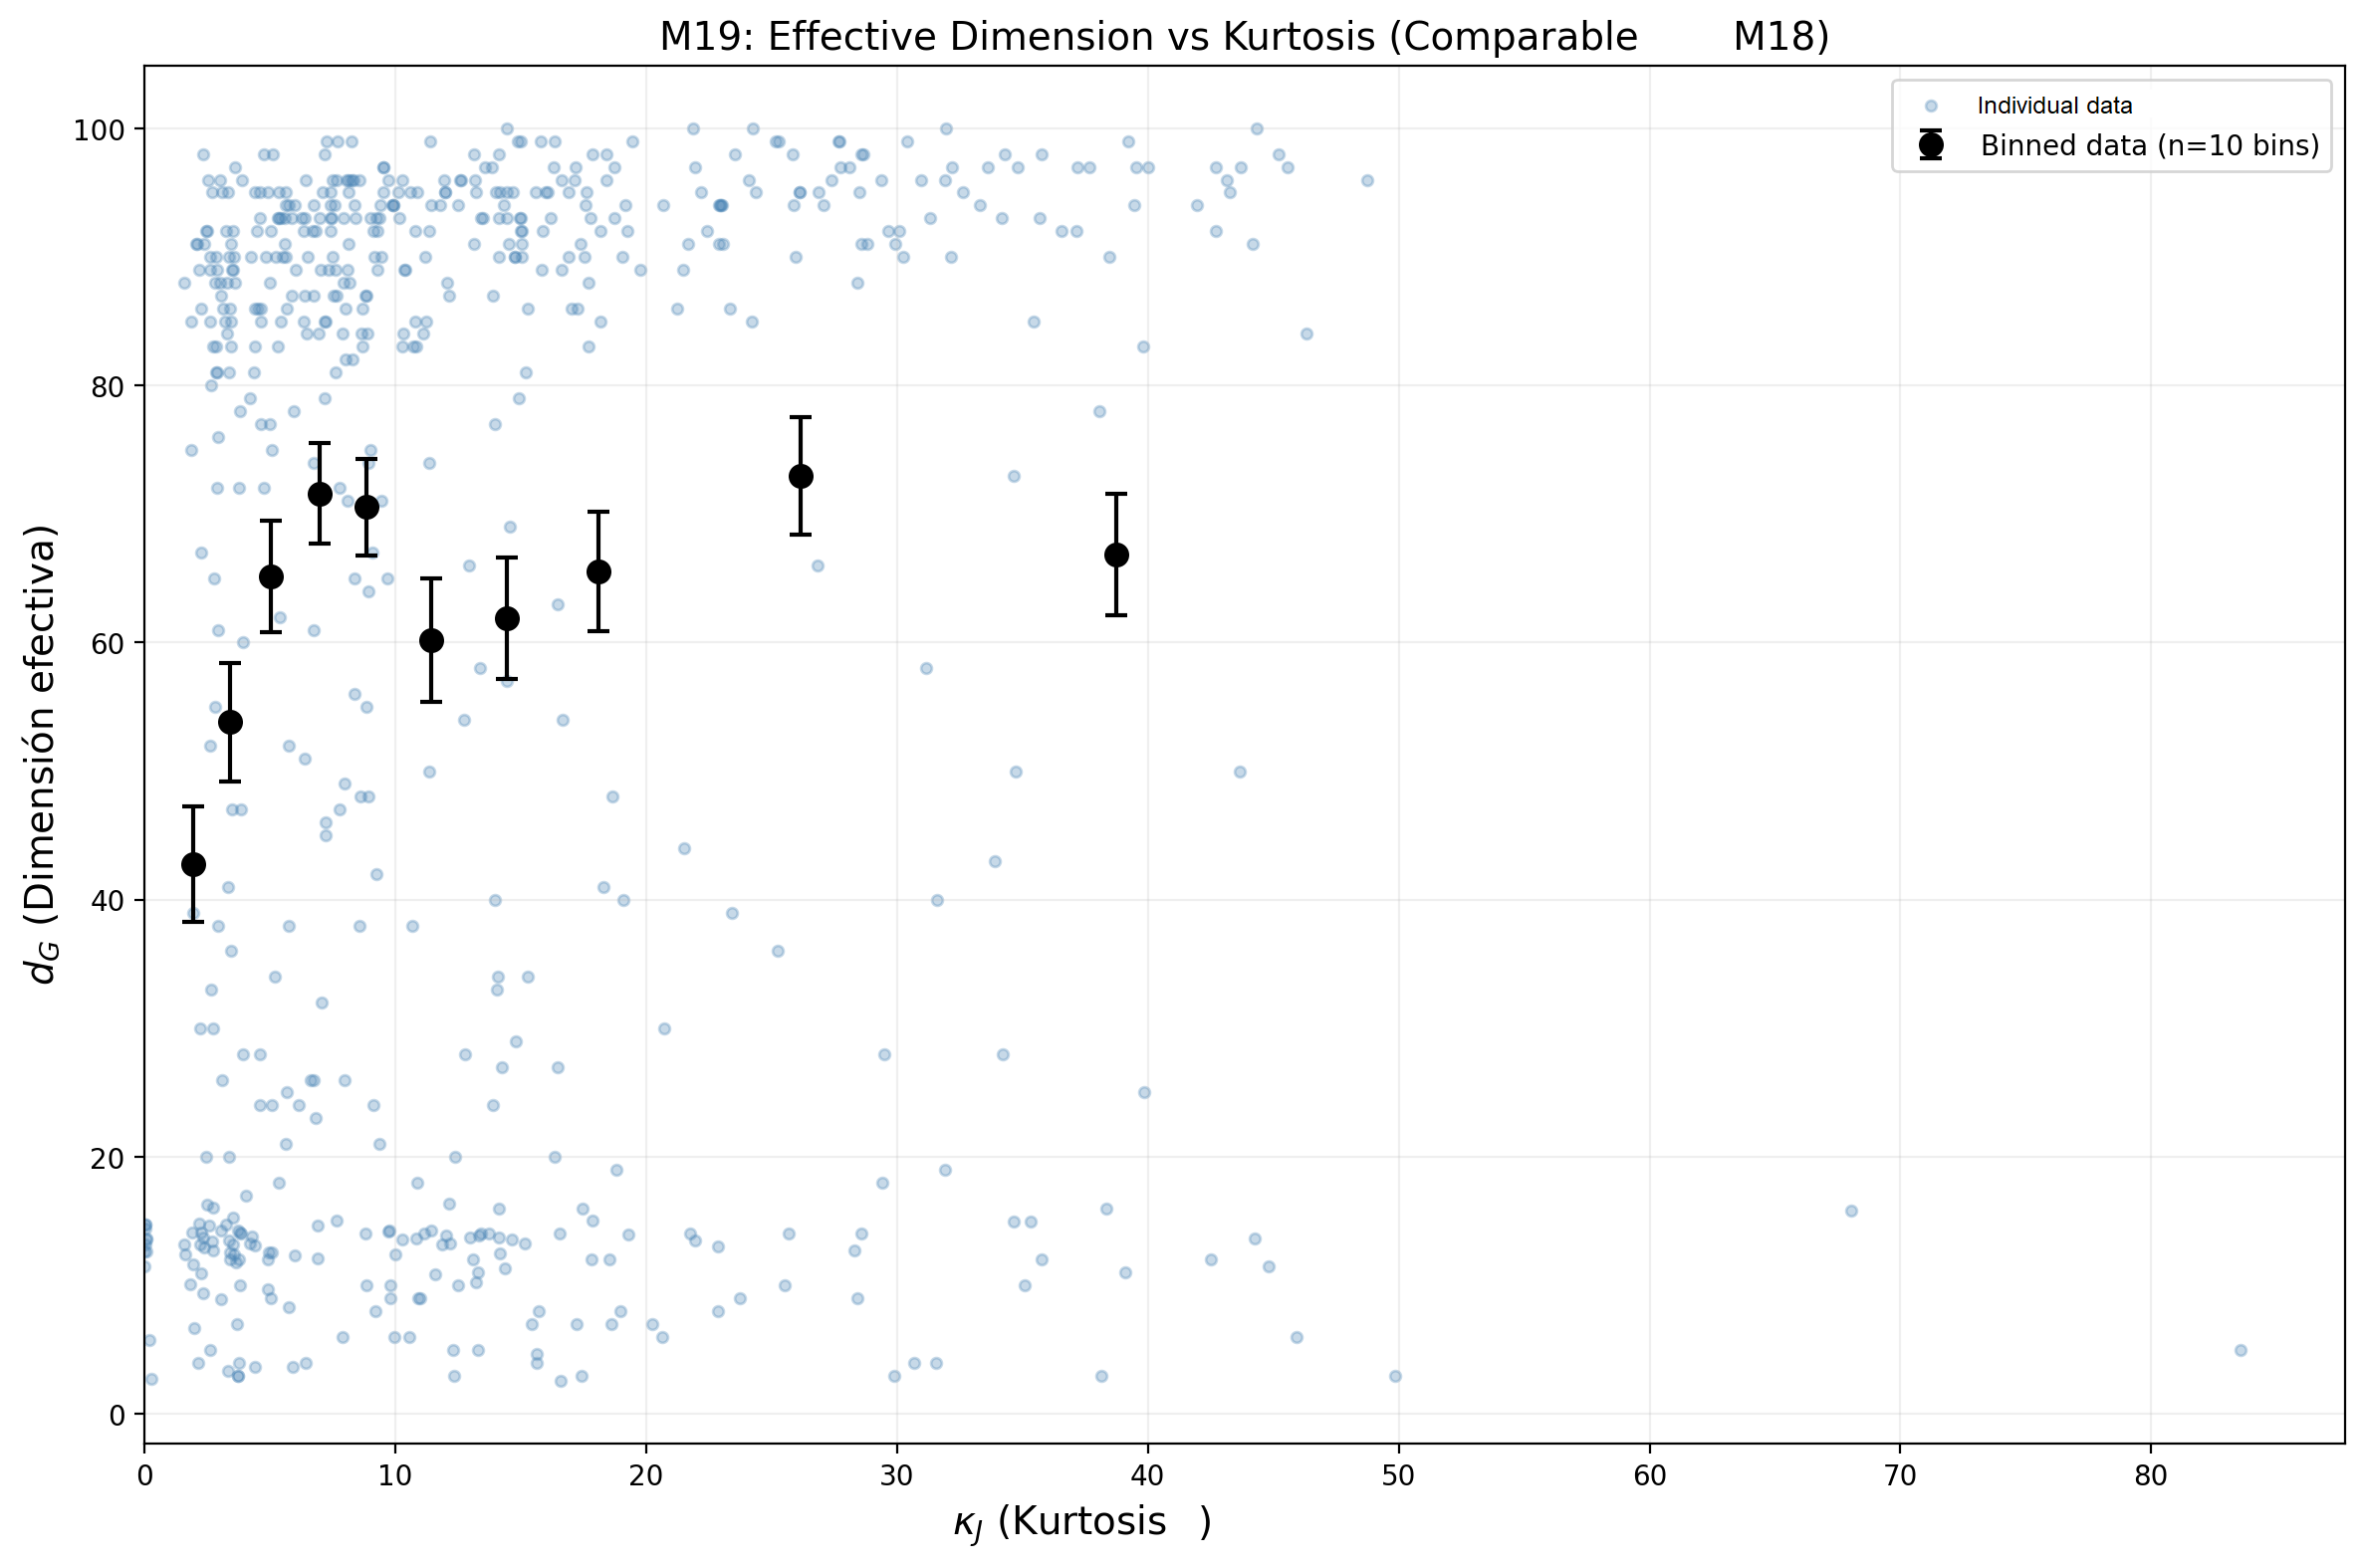
\includegraphics[width=0.8\textwidth]{figures/M19_deff_vs_kappa.png}
\caption{Effective dimensionality vs kurtosis. No sigmoidal transition is observed.}
\end{figure}

Effective dimensionality shows no transition or collapse. Unlike GLG models \citep{gonzalez2023m18}, the system remains structurally invariant, in contrast with the predictions of landscape complexity theory \citep{fyodorov2004complexity, fyodorov2007replica, auffinger2013random}.

\begin{figure}[h!]
\centering
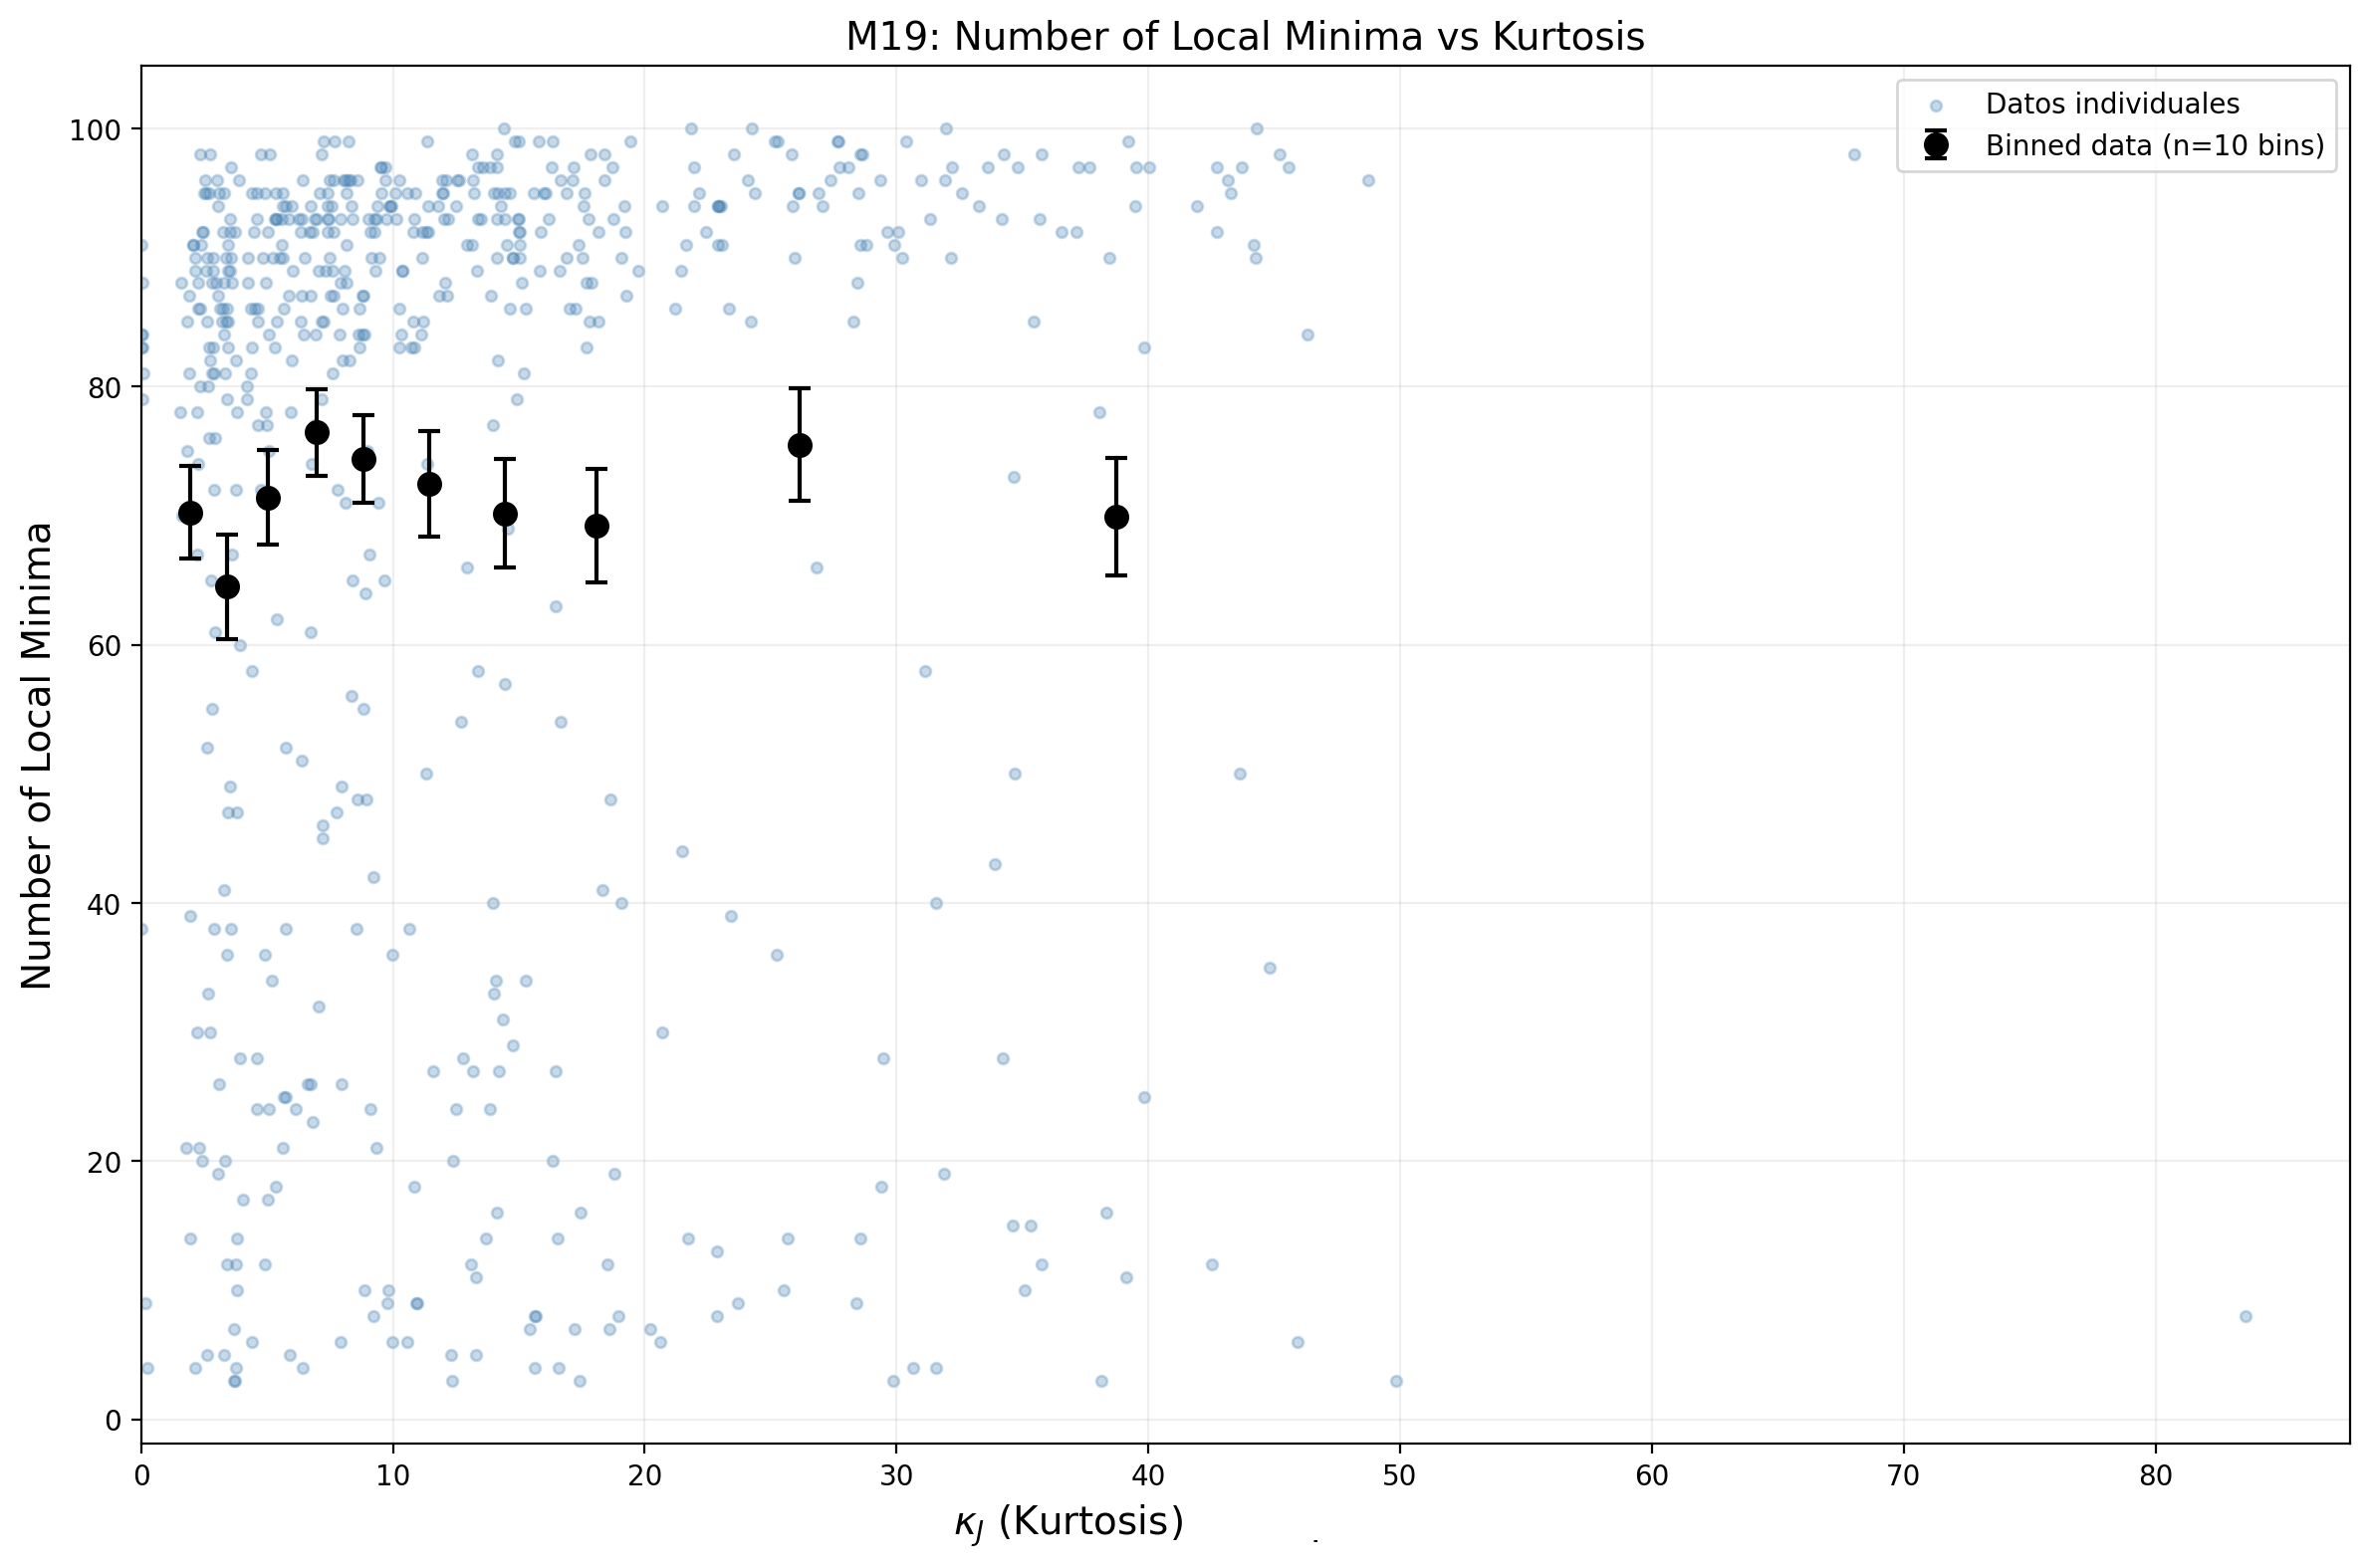
\includegraphics[width=0.8\textwidth]{figures/M19_nmin_vs_kappa.png}
\caption{Number of local minima vs kurtosis. The landscape topology remains stable.}
\end{figure}

The number of local minima remains approximately constant across all kurtosis values, indicating that the diversity of metastable states is not controlled by kurtosis \citep{biroli2000diversity}.

\begin{figure}[h!]
\centering
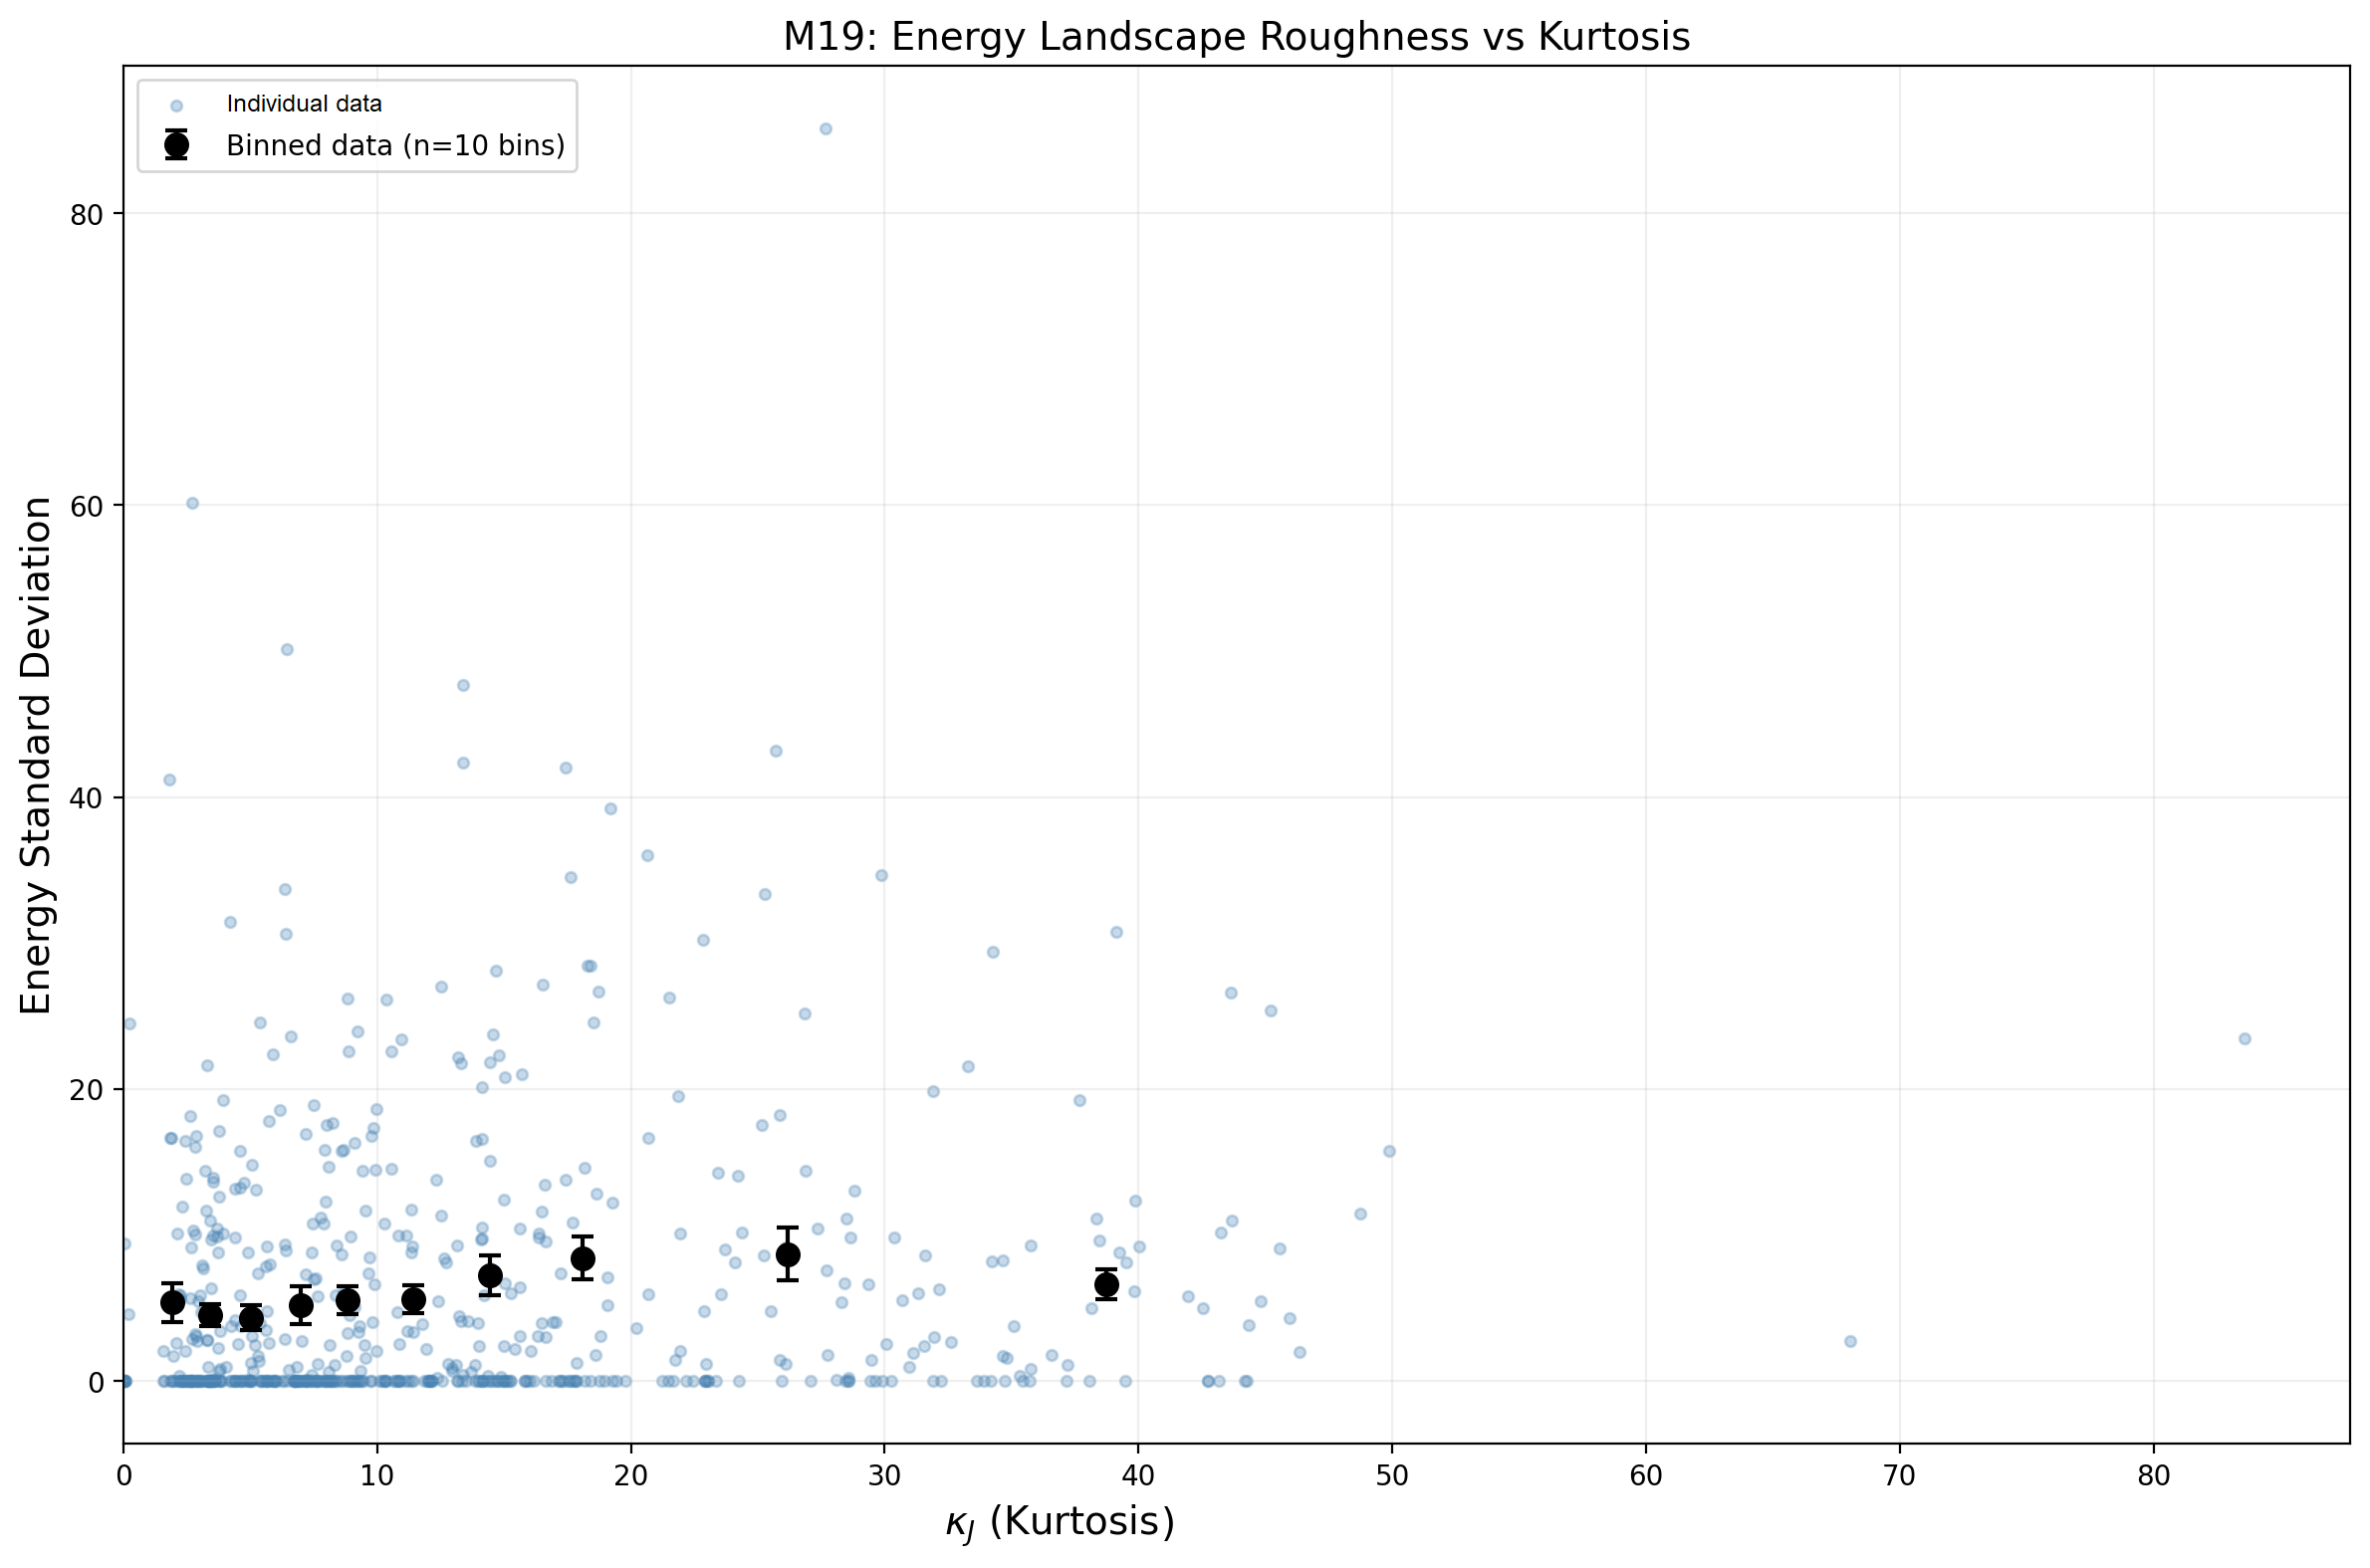
\includegraphics[width=0.8\textwidth]{figures/M19_stdE_vs_kappa.png}
\caption{Energy landscape roughness vs kurtosis. Variance increases slightly but no structural change occurs.}
\end{figure}

Energy fluctuations increase mildly, but without inducing global reorganization.

\subsection{Energy Gap Distributions}

\begin{figure}[h!]
\centering
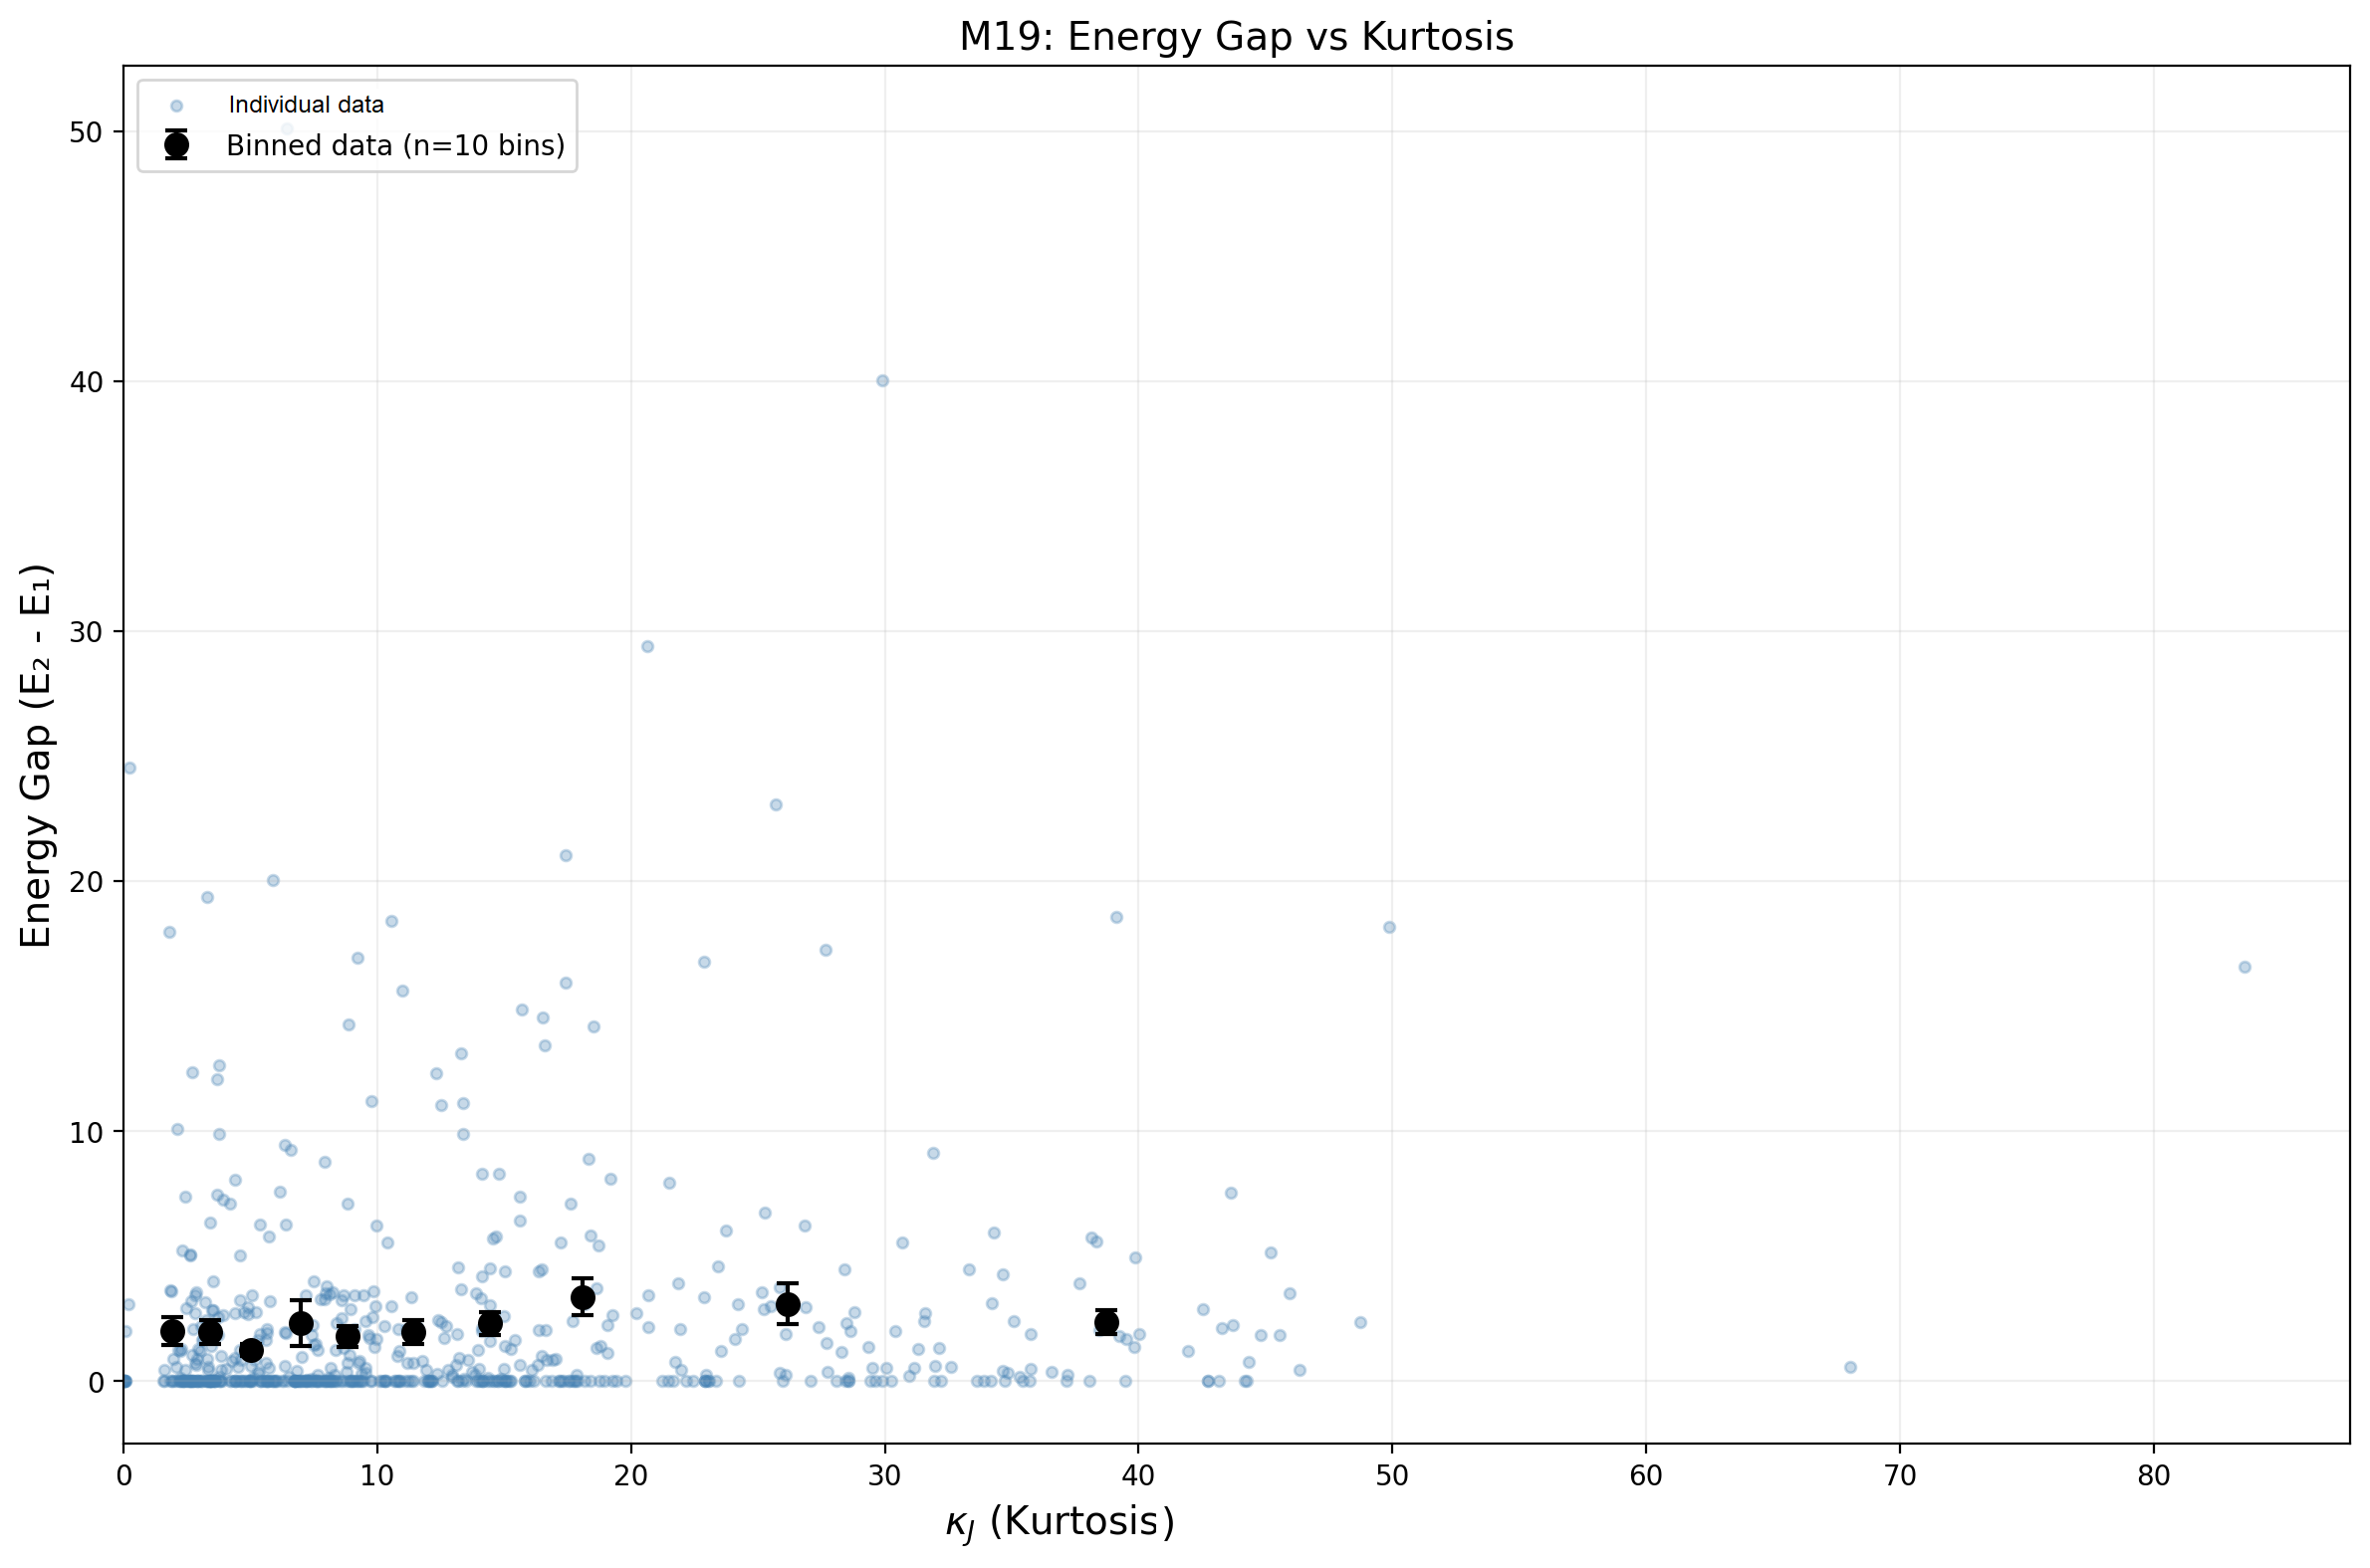
\includegraphics[width=0.8\textwidth]{figures/M19_gap_vs_kappa.png}
\caption{Energy gap vs kurtosis. No characteristic scale emerges.}
\end{figure}

Energy gaps remain broadly distributed, with no clear dependence on kurtosis.

\subsection{Emergence of Heavy Tails}

\begin{figure}[h!]
\centering
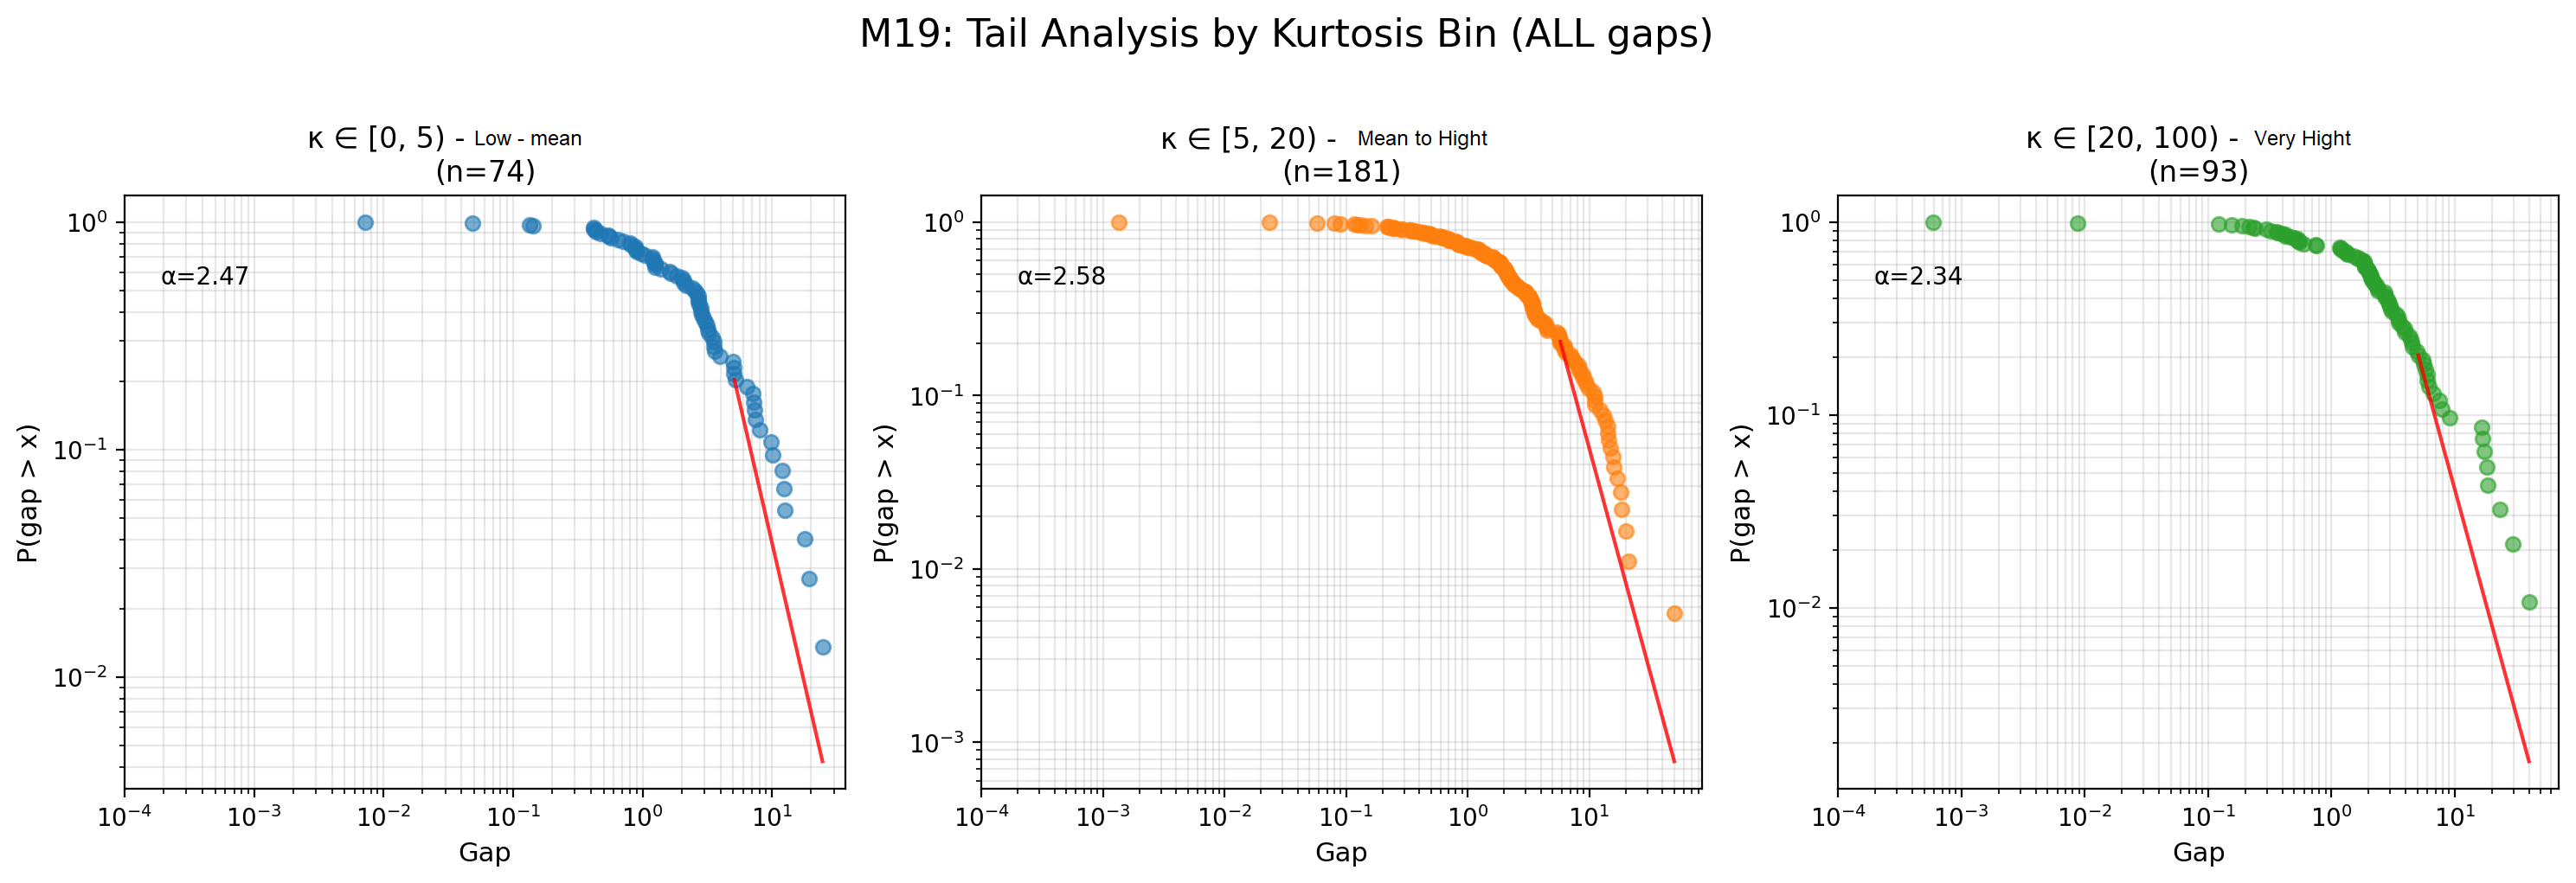
\includegraphics[width=0.9\textwidth]{figures/M19_tail_survival_bins.png}
\caption{Survival functions by kurtosis bin. A transition from log-normal to power-law behavior is observed.}
\end{figure}

At low kurtosis, distributions are compatible with log-normal behavior. At higher kurtosis, clear power-law tails emerge, consistent with the universal extreme-value statistics predicted for disordered systems \citep{bouchaud1997universality}.

\begin{figure}[h!]
\centering
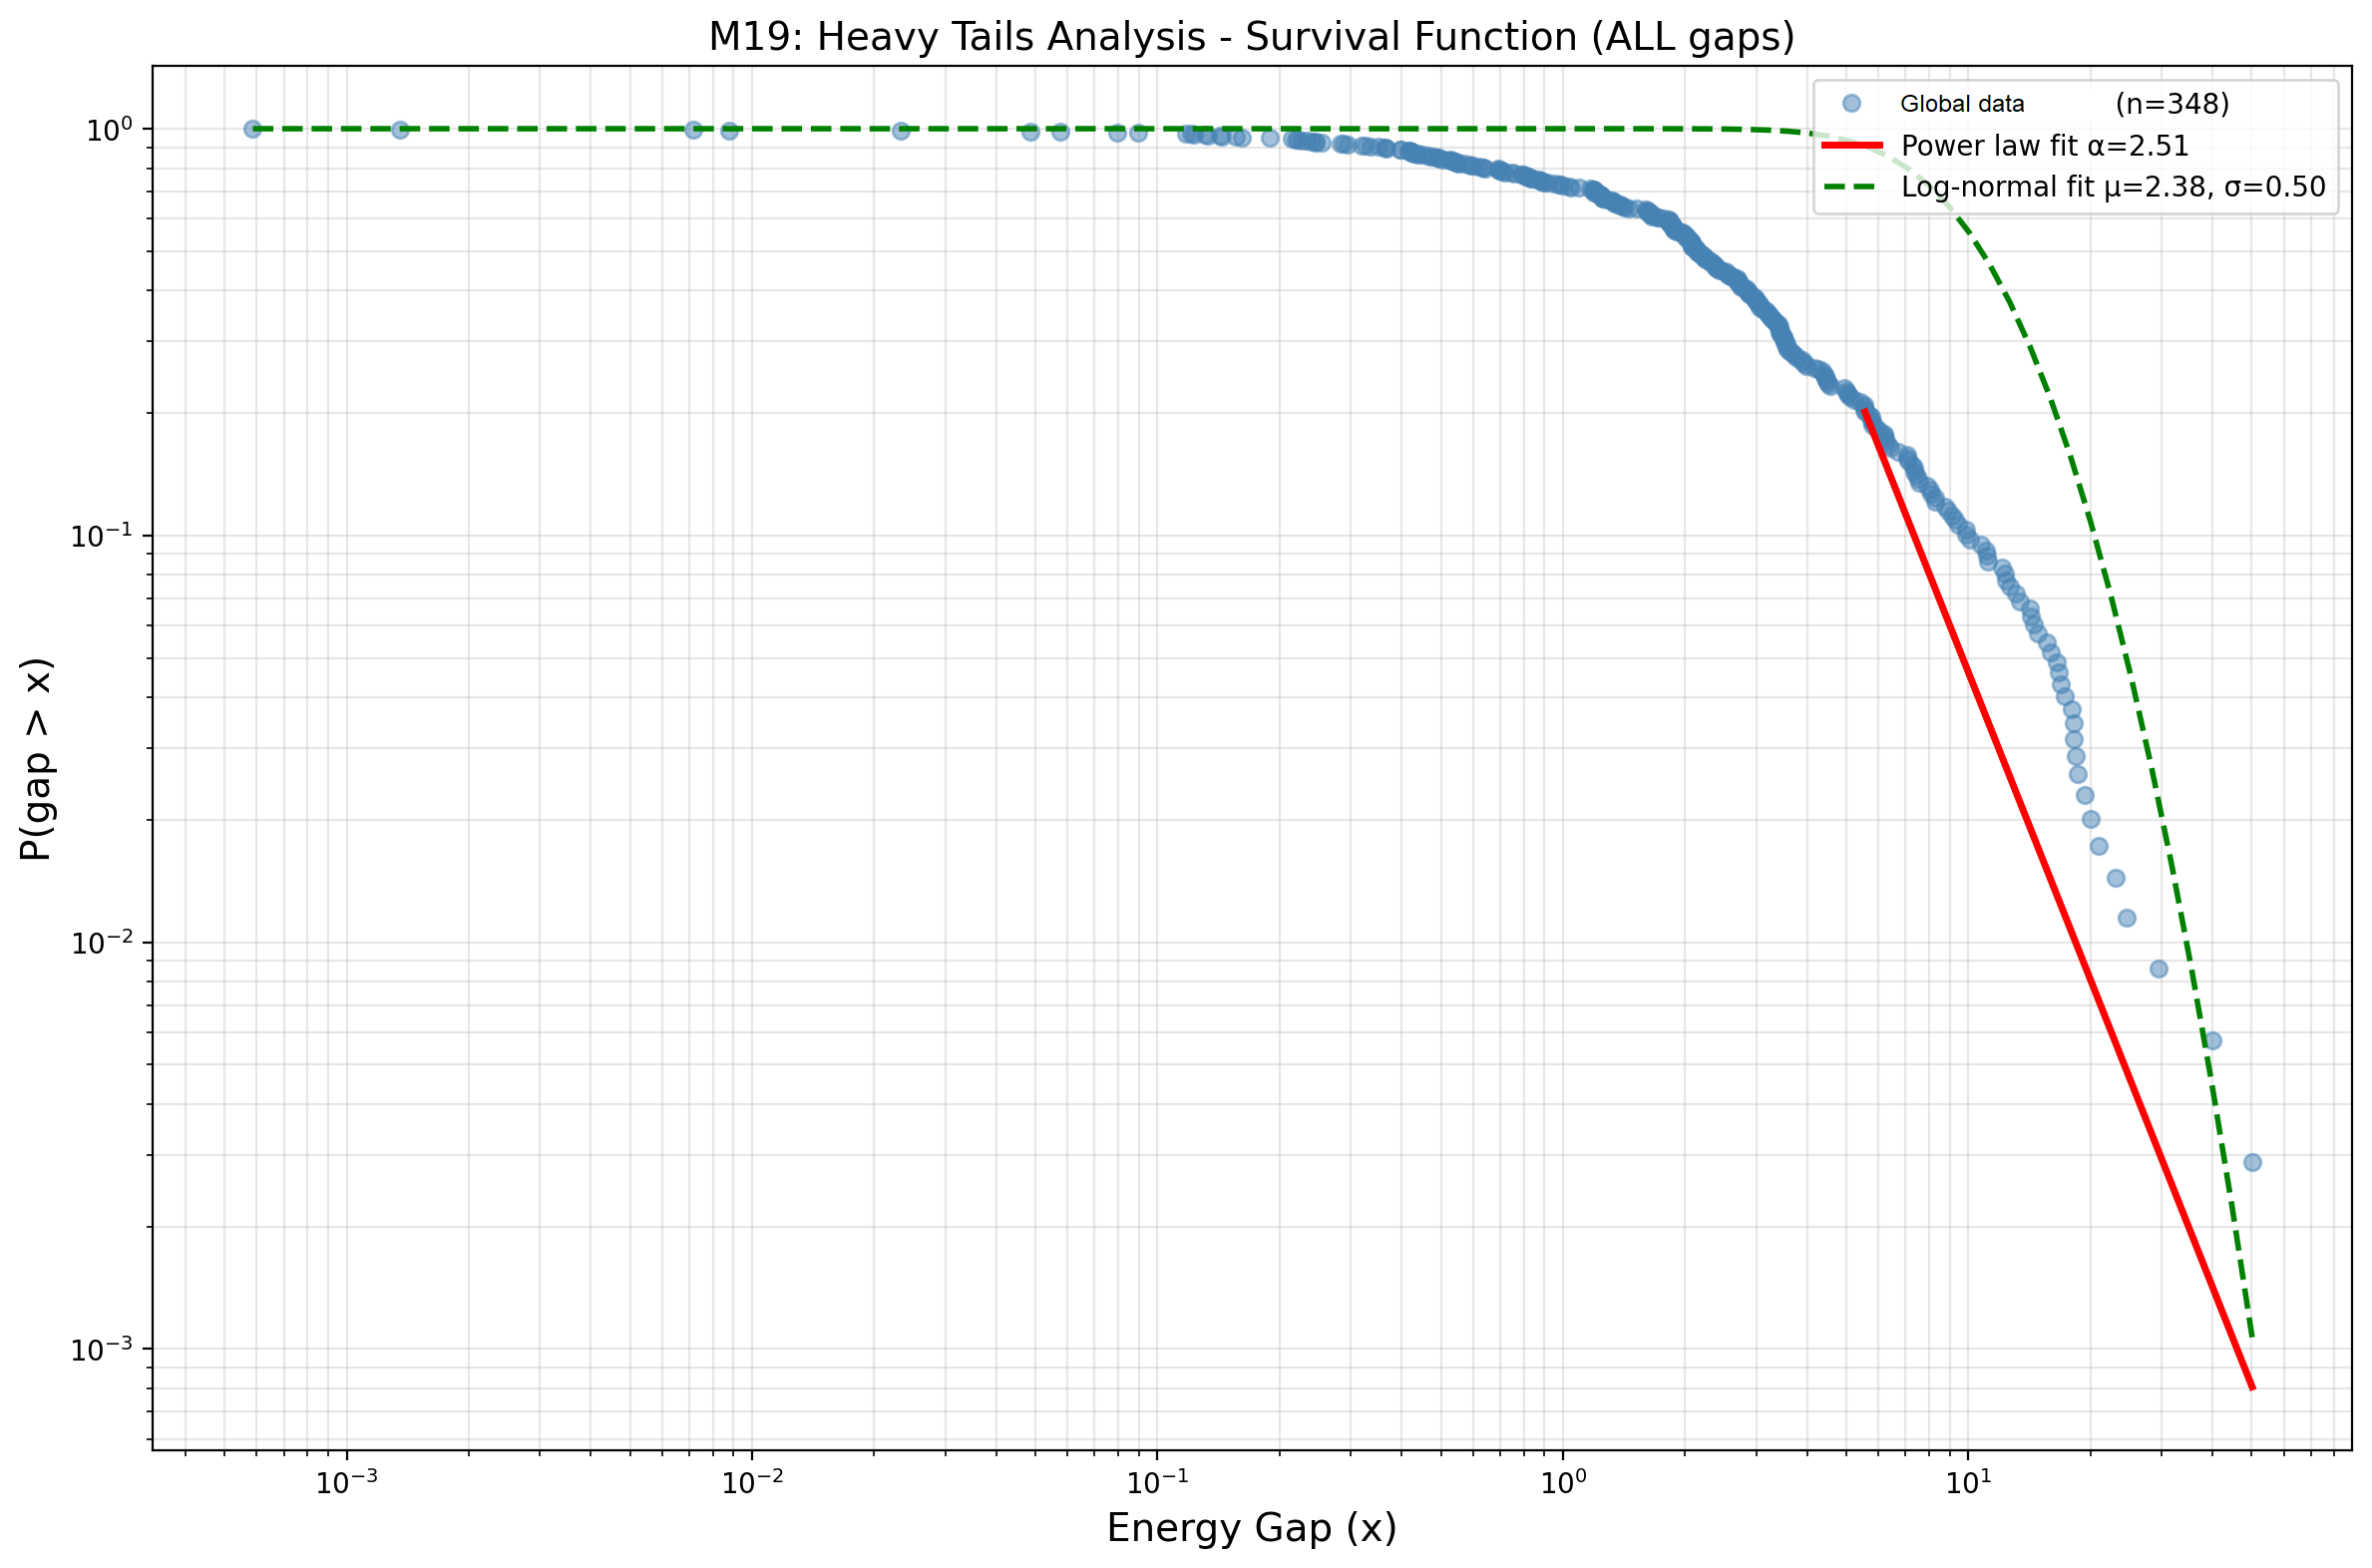
\includegraphics[width=0.8\textwidth]{figures/M19_tail_survival_global.png}
\caption{Global tail analysis. Power law provides the best fit.}
\end{figure}

Global fit results:

\[
\alpha = 2.51, \quad \Delta LL \approx 9.7
\]

indicating a statistically significant preference for a power-law model.

\section{Discussion}

The results demonstrate a clear separation between structural and statistical effects of kurtosis.

\subsection{Failure of Structural Universality}

Unlike GLG systems \citep{gonzalez2023m18}, spin glasses do not exhibit:

\begin{itemize}
\item Sigmoid transitions
\item Dimensional collapse
\item Topological reorganization
\end{itemize}

This shows that kurtosis does not universally control structural emergence, in contrast with theoretical expectations from certain mean-field models \citep{auffinger2013random}.

\subsection{Statistical Transition in Extremes}

However, kurtosis does induce a transition in the statistics of rare events:

\begin{itemize}
\item Low $\kappa$: log-normal-like behavior
\item High $\kappa$: power-law tails
\end{itemize}

This indicates that kurtosis controls:

\[
\text{probability of rare, deep minima}
\]

rather than global structure, a behavior reminiscent of the random energy model's extreme statistics \citep{derrida1980random, derrida1981random}.

\subsection{Mixed Distribution Structure}

The presence of a large mass at zero gaps suggests a mixed distribution:

\begin{itemize}
\item Discrete component: degenerate minima
\item Continuous heavy tail: rare extreme events
\end{itemize}

This structure is characteristic of rugged landscapes with metastability \citep{biroli2000diversity, fyodorov2007replica}.

\section{Conclusion}

We have shown that:

\begin{enumerate}
\item Spin glass systems do not exhibit a kurtosis-driven structural phase transition
\item Kurtosis instead controls the statistics of extreme energy fluctuations
\item A transition from log-normal to power-law tails occurs as kurtosis increases
\end{enumerate}

This establishes a clear limitation of kurtosis-driven universality:

\begin{quote}
Kurtosis induces structural transitions only in systems capable of generative reorganization, but in disordered systems it controls extreme-value statistics instead.
\end{quote}

\section*{Acknowledgments}

This work was developed as part of an independent research program exploring the interface between statistical physics and generative models.

\bibliographystyle{plain}
\bibliography{refs}

\end{document}
